\subsection*{A. Azat’s rounding}

Азату дали задание округлить число вида $1 / n$ до нескольких двоичных знаков после запятой. Например, округляя 
$$1 / 5 = 0{,}2 = 0{,}001100110011..._2$$ 
до 4 цифр после запятой, он получает $0{,}0011_2 = 0{,}1875$. Задача нетривиальная, но зато Азату можно самому выбирать $k$ --- количество знаков после запятой, которые остаются после округления данного ему число. Чтобы было как можно проще, он решил выбрать такое минимальное $k$, чтобы результат округления совпадал с начальным числом. Какое $k$ ему следует выбрать?

\informat{Одно целое число $n$ (от $1$ до $10^{9}$).}

\outformat{Одно целое число $k$. Если такого k не существует, вывести $-1$.}

\examplee{4}{2}{3}{-1}

\excomm{Округляя $1/4 = 0{,}01_2$ до двух знаков после запятой, Вы получаете само число $1/4$.}

\subsection*{B. Billiards}

Чтобы отдохнуть от теории чисел и прочей математики, Димитрий решил сыграть в бильярд на столе шириной $w$ и длиной $h$. Он пускает круглый шар из левого нижнего угла и ждёт, когда он вернётся в тот же угол. Так как Димитрий отдыхает от математики, посчитайте за него, сколько раз шар отразится от горизонтальных и вертикальных бортиков.

\informat{Четыре целых числа $w$, $h$, $x$, $y$ (от 1 до $10^9$), $w$, $h$ --- ширина и длина стола, $(x, y)$ --- вектор скорости, которая была придана шару.}

\outformat{Два целых числа --- количество отражений от горизонтальных и от вертикальных бортиков, соответственно.}
 
\examplee{2 3 \newline 2 2}{3 5}{2 3 \newline 2016 2017}{4033 6047}
 
\excomm{Шар летит с постоянной скоростью, равной начальной. Вектор скорости при отражениях меняется согласно стандартным законам отражения света. Стол не имеет луз и при попадании в угол стола шар просто идёт обратно. Отражение от угла считается отражением от двух бортиков одновременно.}

\subsection*{C. Circles}

Саша любит рисовать круги на клетчатой бумаге. Целым кругом она называет такой круг, у которого центр имеет координаты $(x, 0)$, где $x$ --- целое число, а радиус равен $R$ --- целому положительному числу. Недавно она узнала об очень интересной научной задачке: подсчитать количество точек с целочисленными координатами внутри целого круга. Александра уже развила в себе дух МГУ, и поэтому она ставит более сложную задачу: найти количество целых точек, которые принадлежат сразу двум целым кругам.

\informat{Четыре целых числа $x_1$, $R_1$, $x_2$, $R_2$, где $x_1$ и $x_2$ (от $-10^5$ до $10^5$) --- абсциссы центров двух окружностей, а $R_1$ и $R_2$ (от 1 до $10^5$) --- радиусы окружностей.}
 
\informat{Одно целое число --- количество целых точек внутри пересечения целых кругов.}
 
\examplee{3 4 \newline -1 2}{5}{0 5 \newline 0 13}{81}
  
\subsection*{D. Diners}

Айтмухаммед, Куат и Павел, как и многие другие студенты, после университета добираются домой на автобусах. Сами автобусные маршруты обладают следующими свойствами: 
\begin{itemize}
\item каждая остановка является либо конечной для некоторого маршрута, либо проходной для одного или нескольких маршрутов;
\item все маршруты курсируют от конечных до университета и обратно (маршруты совпадают при движении от университета до дома и обратно).
\item от любой конечной остановки до университета можно добраться только одним маршрутом.
\end{itemize}
Самые отдаленные от университета конечные остановки являются домашними, потому что именно там выходят все студенты, которые едут домой. При этом на каждой домашней остановке обязательно выходит кто-то из студентов. После долгих исследований Илья выяснил, что абсолютно у всех студентов возникает желание перекусить по пути домой. Чтобы удовлетворить желание одногруппников, предприимчивый Илья решил открыть сеть столовых <<Круглый обед>>. Разместить столовые он собирается на остановках, которые находятся ровно на половине пути из университета домой каждого из студентов (если половина пути находится между двумя остановками, то он выберет ближайшую к университету). Где же Илья разметит столовые?
 
\informat{В первой строке одно целое число $n$ (от 2 до 100) --- количество остановок в городе, которые пронумерованы числами от 1 до $n$ (остановка 1 соответствует университету). Во второй строке $(n-1)$ целое число $p_2$, $p_3$, $\dots$, $p_n$ (от 1 до $n$), где $p_k$ --- остановка, на которую едет автобус после остановки $k$ при движении от конечной остановки к университету.}
 
\outformat{Последовательность целых чисел --- номера остановок в порядке возрастания, на которых Илья разместит столовые.}

\examplee{6 \newline 5 1 3 1 1}{3 5}{2 \newline 1}{1}

\excomm{В первом примере студенты выходят на остановках под номерами 2 и 4. Соответственно, столовые разместить надо на 5-й и 3-й остановках.}

\begin{center}
\def\picwidth{0.45\linewidth}
\resizebox{\picwidth}{!}{
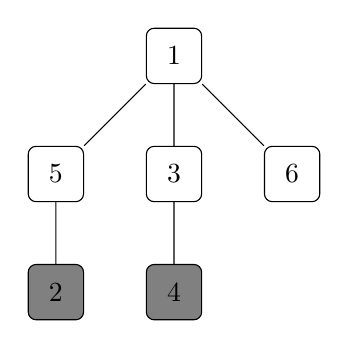
\begin{tikzpicture}[
	every node/.style={
		draw=black, 
		rounded corners=1mm,
		align=center,
		minimum size=20
	}
]
      
\node (T0) {1}
	child {node (T5) {5}
		child {node[fill=gray] (T2) {2}
		}
	}
	child {node (T3) {3}
		child {node[fill=gray] (T4) {4}
		}
	}
	child {node (T6) {6}}
	;
\end{tikzpicture}
}
\end{center}

\subsection*{E. Examination aura}

Аура сессии, которую Ануар постоянно чувствует вокруг себя в университете, подвигла его начать подготовку к экзамену по <<Языкам и методам программирования>>. Ануару необходимо подготовить $n$ билетов. На данный момент его уверенность в понимании $i$-го билета составляет $a_i$ процентов. До экзамена осталось всего k часов, а за 1 час подготовки он может поднять уровень своей уверенности по какому-то одному билету на свой выбор на один процент. Ануара абсолютно не смущает, что он может быть уверен в билете больше, чем на 100 процентов. Да хоть на 256 процентов! Общая уверенность перед экзаменом равна минимальной уверенности среди всех билетов. Какую максимальную общую уверенность перед экзаменом Ануар может гарантировать себе? 
 
\informat{В первой строке два целых числа: $n$ (от 1 до $10^5$) --- количество билетов и $k$ (от 1 до $10^{18}$) --- количество часов до экзамена. \newline
Во второй строке $n$ целых чисел $a_1$, $a_2$, $\dots$, $a_n$ (от 0 до $10^9$) --- уверенность в понимании билетов.}

\outformat{Одно целое число --- максимальная общая уверенность.}
 
\example{5 6 \newline 5 1 4 1 2}{3}
 
\subsection*{F. Fibonaccissimo}
 
Темирхан любит большие числа. Разумеется, он давно знаком с числами Фибоначчи $F_n$, которые, по его словам, с ростом $n$ растут не так быстро, как ему хотелось бы. Чтобы ускорить рост этих чисел, он ввел понятие <<головокружительно больших чисел Фибоначчи>>, где $n$-е число определяется как $F_{F_n}$. Это действительно большие числа! Осталось только придумать, как их вычислять.

\informat{Одно целое число $n$ (от 1 до $10^{18}$).}

\outformat{Одно целое число $F_{F_n}$. Так как ответ может быть очень большим, вывести ответ по модулю $10^9 + 9$}.

\examplee{6}{21}{2017}{372625276}

\subsection*{G. Good round numbers}
 
Бекарыс придумал новый термин --- <<круглость>> числа! Круглостью натурального числа $n$ он называет минимальное такое $k$, для которого найдутся два натуральных числа $p$ и $q$ таких, что $|p - q| = k$ и $p q = n$. Например, круглость точных квадратов равна нулю, что довольно-таки логично. Помогите Бекарысу найти все числа с заданной круглостью на данном отрезке.
 
\informat{Три целых числа $A$, $B$ (от 1 до $10^9$) и $C$ (от 0 до 4).}

\outformat{Одно целое число --- количество чисел с круглостью $C$ на отрезке $[A, B]$}.
 
\examplee{8 32 4}{2}{1 2017 3}{42}


\subsection*{H. Hit a ball}

Игры с мячом, разумеется, полезны для вашего здоровья; вообще, полезны регулярные занятия любым спортом, даже если это никак не относится к данной задаче.
 
\informat{Одно целое число $n$ (от 0 до 10).}

\exampleee{0}{3}{2}{4}{4}{5}

\subsection*{I. Incalculable result}

Тимур и Ерулан недавно узнали, что игры с мячом полезны для здоровья, так что они решили устроить товарищеский теннисный матч между собой. Призом, естественно, является <<Снежный Глобус>>. Правила игры они немного упростили: игра идёт, пока кто-нибудь не наберёт не менее $K$ очков, опережая при этом соперника как минимум на два очка. Нечётные подачи подаёт Тимур, чётные --- Ерулан, то есть, когда кто-то выигрывает очко, подача переходит к следующему игроку. Будем говорить, что произошла неожиданность, если игрок выиграл очко на подаче соперника. Тимур и Ерулан при этом записали номера подач, на которых возникали неожиданности. Восстановите число подач в данной игре.
 
\informat{В первой строке два целых числа: $N$ (от 1 до 100) и $K$ (от 1 до 100), число неожиданностей и минимальное количество очков, нужное для победы, соответственно. \newline
Во второй строке $N$ целых чисел (от 1 до 1000) --- номера подач, на которых произошли неожиданности.}

\outformat{Одно целое число --- количество подач в данной партии. Если партия не могла развиваться по описанному сценарию, то вывести -1.}

\exampleee{3 6 \newline 1 4 5}{10}{4 10 \newline 1 4 7 10}{-1}{2 2 \newline 1 2}{-1}

\excomm{В первом примере выигрывает Ерулан со счётом 6:4, взяв очки на своих подачах 2, 6, 8, 10 и на чужих под номерами 1 и 5. \newline
Во втором примере никто никогда не наберёт на два очка больше соперника, поскольку после десятой подачи при счёте 5:5 Тимур и Ерулан начинают брать очки поочерёдно.}
